\documentclass{standalone}
\usepackage{tikz}

\begin{document}

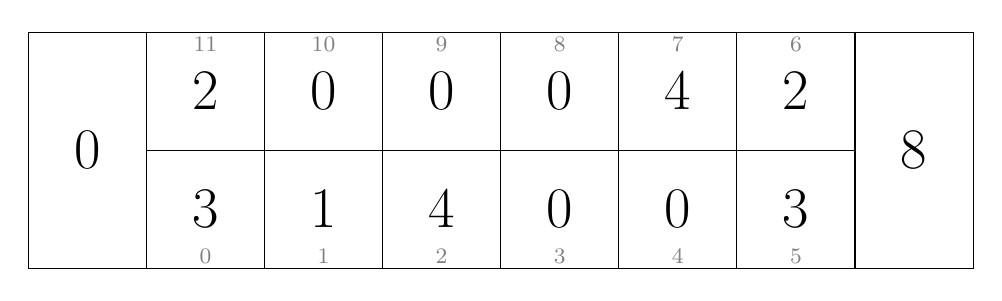
\begin{tikzpicture}[scale=1.5, font=\huge]
% Cases
\foreach \x/\stones/\label in {0/3/0,1/1/1,2/4/2,3/0/3,4/0/4,5/3/5} {
  \draw (\x,0) rectangle ++(1,1) node[pos=.5] {\stones};
  \draw (\x+0.5,0.1) node[text=gray, font=\footnotesize] {\label};
}
\foreach \x/\stones/\label in {5/2/6,4/4/7,3/0/8,2/0/9,1/0/10,0/2/11} {
  \draw (\x,1) rectangle ++(1,1) node[pos=.5] {\stones};
  \draw (\x+0.5,1.9) node[text=gray, font=\footnotesize] {\label};
}
% Grands magasins
\draw (-1,0) rectangle ++(1,2) node[midway] {0};
\draw (6,0) rectangle ++(1,2) node[midway] {8};
\end{tikzpicture}

\end{document}

